\documentclass[12pt]{article}
\usepackage[utf8]{inputenc}
\usepackage{geometry}
\geometry{letterpaper, margin=0.25in}
\usepackage{graphicx} 
\usepackage{parskip}
\usepackage{booktabs}
\usepackage{array} 
\usepackage{paralist} 
\usepackage{verbatim}
\usepackage{subfig}
\usepackage{fancyhdr}
\usepackage{sectsty}
\usepackage[shortlabels]{enumitem}

\pagestyle{fancy}
\renewcommand{\headrulewidth}{0pt} 
\lhead{}\chead{}\rhead{}
\lfoot{}\cfoot{\thepage}\rfoot{}

%%% ToC (table of contents) APPEARANCE
\usepackage[nottoc,notlof,notlot]{tocbibind} 
\usepackage[titles,subfigure]{tocloft}
\renewcommand{\cftsecfont}{\rmfamily\mdseries\upshape}
\renewcommand{\cftsecpagefont}{\rmfamily\mdseries\upshape} %

\usepackage{amsmath}
\usepackage{amssymb}
\usepackage{mathtools}
\usepackage{empheq}
\usepackage{xcolor}
\usepackage{bbm}
\usepackage{tikz}
\usepackage{pgfplots}
\usepackage{tikz-cd}
\pgfplotsset{compat=1.18}

\newcommand{\ans}[1]{\boxed{\text{#1}}}
\newcommand{\vecs}[1]{\langle #1\rangle}
\renewcommand{\hat}[1]{\widehat{#1}}

\renewcommand{\P}{\mathbb{P}}
\newcommand{\R}{\mathbb{R}}
\newcommand{\E}{\mathbb{E}}
\newcommand{\Z}{\mathbb{Z}}
\newcommand{\N}{\mathbb{N}}
\newcommand{\Q}{\mathbb{Q}}
\newcommand{\C}{\mathbb{C}}

\newcommand{\ind}{\mathbbm{1}}
\newcommand{\qed}{\quad \blacksquare}

\newcommand{\brak}[1]{\left\langle #1 \right\rangle}
\newcommand{\bra}[1]{\left\langle #1 \right\vert}
\newcommand{\ket}[1]{\left\vert #1 \right\rangle}

\newcommand{\abs}[1]{\left\vert #1 \right\vert}
\newcommand{\norm}[1]{\left\vert\left\vert #1 \right\vert\right\vert}

\newcommand{\mfX}{\mathfrak{X}}
\newcommand{\ep}{\varepsilon}

\newcommand{\Ec}{\mathcal{E}}
\newcommand{\A}{\mathcal{A}}
\newcommand{\F}{\mathcal{F}}
\newcommand{\Cc}{\mathcal{C}}
\newcommand{\B}{\mathcal{B}}
\newcommand{\M}{\mathcal{M}}
\newcommand{\X}{\chi}
\renewcommand{\L}{\mathcal{L}}

\newcommand{\sub}{\subseteq}
\newcommand{\st}{\text{ s.t. }}
\newcommand{\card}{\text{card }}
\renewcommand{\div}{\vspace*{10pt}\hrule\vspace*{10pt}}
\newcommand{\surj}{\twoheadrightarrow}
\newcommand{\inj}{\hookrightarrow}
\newcommand{\biject}{\hookrightarrow \hspace{-8pt} \rightarrow}
\renewcommand{\bar}[1]{\overline{#1}}
\newcommand{\overcirc}[1]{\overset{\circ}{#1}}
\newcommand{\diam}{\text{diam }}

\renewcommand{\Re}{\text{Re}\,}
\renewcommand{\Im}{\text{Im}\,}
\newcommand{\sign}{\text{sign}\,}

\newcommand{\iid}{\overset{\text{iid}}{\sim}}
\newcommand*{\tbf}[1]{\ifmmode\mathbf{#1}\else\textbf{#1}\fi}

\DeclareMathOperator*{\argmax}{\arg\max}
\DeclareMathOperator*{\argmin}{\arg\min}


\usepackage{tcolorbox}
\tcbuselibrary{breakable, skins}
\tcbset{enhanced}
\newenvironment*{tbox}[2][gray]{
    \begin{tcolorbox}[
        parbox=false,
        colback=#1!5!white,
        colframe=#1!75!black,
        breakable,
        title={#2}
    ]}
    {\end{tcolorbox}}

\newenvironment*{exercise}[1][red]{
    \begin{tcolorbox}[
        parbox=false,
        colback=#1!5!white,
        colframe=#1!75!black,
        breakable
    ]}
    {\end{tcolorbox}}

\newenvironment*{proof}[1][blue]{
\begin{tcolorbox}[
    parbox=false,
    colback=#1!5!white,
    colframe=#1!75!black,
    breakable
]}
{\end{tcolorbox}}

\title{APMA 1740: Recent Applications of Probability and Statistics}
\author{Milan Capoor}
\date{Spring 2025}

\begin{document}
\maketitle

\section{Jan 22}
\subsection{Maximum Entropy Principle}
\tbf{A strange though experiment of Gibbs:} Imagine a physical system $S$ (say a gas) in an ``infinite bath''. Let $x$ be the state of every particle (positions, velocities, ...) in $S$.

For simplicity, let $S$ be be $3$ particles in $\Z^2$ with $x \in \Z^6$ being the positions. Let $s$ be the number of states of particles in $S$.

\emph{What is $p(x)$, the probability that $S$ has state $x$?}

In the simplest case (each particle is independent and the state distribution is uniform), we trivially have $P(x) = \frac{1}{s}$. But in general, these are incredibly strong assumptions.

We can create some constraints to do better.

\begin{enumerate}
    \item Assume that the average kinetic energy $\Ec$ of the infinite heat bath is some constant $\theta$.

          In this case, we expect the average kinetic energy of $S$ is approximately $\theta$:
          \[\sum_x  p(x) \Ec(x) = \theta\]

    \item Trivially, $p$ is a probability distribution, so
          \[\sum_x p(x) = 1\]
\end{enumerate}

But still this is far from enough: this gives us only $2$ constraints for $s$ many unknowns!

However, we can approximate with the LLN. Sample $n \gg s \gg 1$ iid copies of $S$, $S_1, S_2, \dots, S_n$ with positions $x_1, x_2, \dots, x_n$.

Define the \tbf{empirical distribution}
\[\hat p_x = \frac{\#\{i: X_i = x\}}{n}\]

So with large $n$, $\hat p = p$, and
\[\sum_x \hat p(x) \Ec(x) \approx \theta\]

\emph{Claim:} The vast majority of assignments of states to $X_1, \dots, X_n$ yield a single empirical distribution $\hat p$.

Consider $C(\hat p)$, the number of ways to assign a state to each of $n$ systems that would yield $\hat p$. Then, with $\hat n_x = \hat p_x \cdot n = \#\{i: X_i = x\}$,
\[\textcolor{red}{C(\hat p) = \binom{n}{\prod_{i=1}^s n_i}}\]

\section{Jan 24}
\tbf{Recall:} For a system $S$ with $s$ states, what is the probability $p(x)$ that $S$ is in state $x$?

We know that $\sum_{x=1}^s p(x) = 1$ and $\sum_{x=1}^s p(x) \Ec(x) = \theta$ for some constant $\theta$.

We sample $X_1, \dots, X_n$ iid from $S$ ($n \gg s\gg 1$) and define the empirical distribution $\hat p_x = \frac{\#\{i: X_i = x\}}{n}$. By LLN, $\hat p \approx p$.

\tbf{Claim:} $\hat p$ should maximize $C(\hat p)$, the number of arrangements of $n$ states $\{1, \dots, s\}$ that yield $\hat p$:
\[C(\hat p) = \binom{n}{\hat p_1 n\dots \hat p_s n} = \frac{n!}{(\hat p_1 n)! \dots (\hat p_s n)!}\]
where $\hat p_i n$ is the number of times we see state $i$ in the sample.

\emph{Example:} For $s = 2$, put $n$ balls into $2$ bins $\{1, 2\}$. Then $\hat p_1 n = a$ balls in bin 1, $\hat p+2 n = n- a$ balls in bin 2. We write this
\[C(\hat p) = \binom{n}{a} = \binom{n}{a, n-a} = \frac{n!}{a!(n-a)!}\]

\tbf{Stirling's Approximation:}
\[k! \approx \frac{k^k}{e^k} \sqrt{2\pi k}\]

Hence,
\begin{align*}
    C(\hat p)                  & = \frac{n^n e^{-n} \sqrt{2\pi n}}{\prod_{i=1}^s (\hat p_i n)^{\hat p_i n} e^{-\hat p_i n} \sqrt{2\pi \hat p_i n}}                           \\
    \log C(\hat p)             & = n\log n - n + \log\sqrt{2\pi n} -\sum_{i=1}^s \left[\hat p_i n \log (\hat p_i n) - \hat p_i n + \log \sqrt{2\pi n}\right]                 \\
    \frac{1}{n} \log C(\hat p) & = \log n - 1 + \frac{1}{n}\log\sqrt{2\pi n}-\sum_{i=1}^s \left[\hat p_i \log (\hat p_i n) - \hat p_i + \frac{1}{n}\log \sqrt{2\pi n}\right] \\
                               & = \log n - \frac{1}{n}\log\sqrt{2\pi n}-\sum_{i=1}^s \left[\hat p_i \log (\hat p_i) + \frac{1}{n}\log \sqrt{2\pi n}\right]                  \\
                               & = -\sum_{i=1}^s \hat p_i \log \hat p_i - \frac{1}{n} \sum_{i=1}^s \log \sqrt{2\pi \hat p_i n} + \frac{1}{n}\log \sqrt{2\pi n}
\end{align*}

Since, $\hat p_i \leq 1$, $\frac{1}{n} \log \sqrt{2\pi \hat p_i n} \leq \log n$. Further, $\frac{\log n}{n} \to 0$ so
\[\frac{1}{n} \log C(\hat p) \approx -\sum \hat p_i \log \hat p_i\]

\tbf{Definition:} If $p$ is a probability distribution, its \tbf{Shannon Entropy} is
\[H(p) = \sum p(x) \log \frac{1}{p(x)} = -\sum p(x) \log p(x)\]

\emph{Note:} $H(p) \geq 0$ since $p(x) \leq 1$ for all $p$.

Back to our original problem, we seek $\hat p$ that satisfies
\begin{itemize}
    \item $\sum_{x=1}^s \hat p_x = 1$
    \item $\sum_{x=1}^s \hat p_x \Ec(x) \approx \theta$
    \item $\hat p$ maximizes $C(\hat p)$, i.e. maximizes Shannon Entropy $H(\hat p)$
\end{itemize}

We turn to our trusty friend, Lagrange multipliers. We seek to chose $p$ to maximize
\[H(p) + \gamma \sum_{x=1}^s p_x + \lambda \sum_{x=1}^s p_x \Ec(x)\]

Taking derivatives WRT $p_x$,
\begin{align*}
    \frac{\partial}{\partial p_x} \left[H(p) + \gamma \sum_{x=1}^s p_x + \lambda \sum_{x=1}^s p_x \Ec(x)\right] & = \frac{\partial}{\partial p_x} \left[-\sum_x p_x \log p_x\right] +\gamma + \lambda \Ec(x) \\
                                                                                                                & = -\log p_x - 1 + \gamma + \lambda \Ec(x) = 0
\end{align*}

So $\gamma + \lambda \Ec(x) - 1 = \log p(x)$ and
\begin{align*}
    p(x) & = e^{-1} e^{\lambda \Ec(x)} e^{\gamma + \lambda \Ec(x)} \\
         & = \frac{1}{z_{\lambda}} e^{\lambda \Ec(x)}
\end{align*}
where $Z_{\lambda} = \sum_{x=1}^s e^{\lambda \Ec(x)}$.

To find $\lambda$, we use the constraint $\sum p_{x} \Ec(x) \theta$.

\section{Jan 27}
\tbf{Example:} Find the maximum entropy distribution $p$ on $\{1, 2, 3\}$ (i.e. $s = 3$) satisfying $\E_p X^2 = 2$, i.e. $\sum_{x=1}^s p_x x^2 = 2$.

Since $\E_p X^2 = \sum_{x=1}^s p(x) x^2 = 2$, $\Ec(x) = x^2$,
\[p(x) = \frac{1}{Z} e^{\lambda \Ec(x)} = \frac{1}{Z} e^{\lambda x^2}, \quad x = 1, 2, 3\]

We need to find $Z, \lambda$ satisfying
\begin{itemize}
    \item $\E_p X^2 = 2$
    \item $\sum p_x = 1$
\end{itemize}

Hence,
\begin{align*}
    \begin{cases}
        \frac{1}{Z}[e^{\lambda} + 4e^{4\lambda} + 9e^{9\lambda}] = 2 \\
        \frac{1}{Z}[e^{\lambda} + e^{4\lambda} + e^{9\lambda}] = 1
    \end{cases} & \implies Z = e^{\lambda} + e^{4\lambda} + e^{9\lambda}                                                                                                         \\
                                                                                                                       & \implies e^{\lambda} + 4e^{4\lambda} + 9e^{9\lambda} = 2(e^{\lambda} + e^{4\lambda} + e^{9\lambda}) \\
                                                                                                                       & \implies e^{\lambda} - 2e^{4\lambda} - 7e^{9\lambda} = 0
\end{align*}

We can solve for $\lambda$ with any numeric method.


\subsection{Maximum Entropy Principle in the Continuum}
\tbf{Definition:} Let $p$ be a PDF. Its \tbf{entropy} is defined as
\[H(p) = -\int_{-\infty}^{\infty} p(x) \log p(x)\; dx\]

\tbf{Example (MEP with multiple constraints):} Find $p$ that maximizes $H(p)$ subject to
\[\begin{cases}
        \sum p_x \Ec_1(x) = \theta_1 \\
        \vdots                       \\
        \sum p_x \Ec_k(x) = \theta_k \\
        \sum p_x = 1
    \end{cases}\]

Our Lagrange multipliers are given by
\[\max\left[H(p) + \lambda_1 \sum p_x \Ec_1(x) + \lambda_2 \sum p_x \Ec_2(x) + \dots + \lambda_k \sum p_x \Ec_k(x) + \gamma \sum p_x\right]\]

Taking derivatives WRT $p_x$, we get
\begin{align*}
    H(p) & = -\log p_x - 1 + \lambda_1 \Ec_1(x) + \dots + \lambda_k \Ec_k(x) + \gamma = 0              \\
         & \implies p_x = \frac{1}{Z} \exp\left[\lambda_1 \Ec_1(x) + \dots + \lambda_k \Ec_k(x)\right]
\end{align*}

The rest follows as before.

\tbf{Example:} Find the max entropy density subject to $\E_p X^2 = 1$ and $\E_p X = 0$.

In this case,
\[p_x = \frac{1}{Z} \exp\left[\lambda_1 \Ec_1(x) + \lambda_2 \Ec_2(x)\right]\]
where
\[\Ec_1(x) = x^2, \quad \Ec_2(x) = x\]

Hence, we have constraints
\[\begin{cases}
        \frac{1}{Z} \left[\int_{-\infty}^{\infty} e^{\lambda_1 x^2 + \lambda_2 x} x^2\; dx\right] = 1 \\
        \frac{1}{Z} \left[\int_{-\infty}^{\infty} e^{\lambda_1 x^2 + \lambda_2 x} x\; dx\right] = 0   \\
        \frac{1}{Z} \left[\int_{-\infty}^{\infty} e^{\lambda_1 x^2 + \lambda_2 x}\; dx\right] = 1
    \end{cases}\]

We can complete the square to get the integrals in the forms of a Gaussian:
\[\frac{1}{Z}e^{\lambda_1 x^2  +\lambda_2 x} = \frac{1}{Z}\exp\left[\lambda_1 \left(x - \frac{\lambda_2}{2\lambda_2}\right)^2 \right] \sim N(\frac{\lambda_2}{2\lambda_1}, \frac{-1}{2\lambda_1})\]

But we have mean $0$ and variance $1$ so
\[\frac{\lambda_2}{2\lambda_1} = 0 \implies \lambda_2 = 0, \quad -\frac{1}{2\lambda_1} = 1 \implies \lambda_1 = -\frac{1}{2}\]

$Z$ follows from simply computing
\[Z = \int_{-\infty}^{\infty} \exp(\lambda_1 x^2 + \lambda_2 x)\; dx\]

\subsection{Large Deviation Principle}

\begin{tbox}{\textbf{Large Deviation Principle:} Take $p$ on $\{1, 2, \dots, s\}$, $\Ec: \{1, \dots, s\} \to \R$. Observe $X_1, X_2, \, \dots,\, X_n \overset{\text{iid}}{\sim} p$. Define
        \[\frac{1}{n}\sum_{x=1}^n \Ec(X_k) = \theta\]. Define the empirical distribution $\hat p_x = \frac{1}{n}\cdot \#\{i: X_i = x\}$. Then $\E_{\hat p}\, \Ec(X) = \theta$}

    \emph{Proof:}
    \begin{align*}
        \E_{\hat p}\, \Ec(X) & = \sum_{x=1}^s \hat p_x \Ec(x)                                   \\
                             & = \frac{1}{n}\sum_{x=1}^s \Ec(x) \sum_{i=1}^n \ind_{X_i}         \\
                             & = \frac{1}{n}\sum_{i=1}^n \sum_{x=1}^s \ind_{X_i=x} \cdot \Ec(x) \\
                             & = \frac{1}{n} \sum_{i=1}^{n} \Ec(X_i) = \theta
    \end{align*}
\end{tbox}

Let $q$ be some probability distribution on $\{1, \dots, s\}$. What is $\P(\hat p = q)$?

Recall that the $C(\hat p)$ function gave the number of ways to assign a state to each of $n$ systems that would yield $\hat p$. Similarly, here we have
\[\P(\hat p = q) = \binom{n}{n_1 \cdots n_s} \prod_{x=1}^s p_x^{q_x \cdot n}\]

\tbf{Example:} Take $X_1, X_2 \sim p$. Let $q = \frac{1}{2} \delta_\{1\} + \frac{1}{2} \delta_\{2\}$. What is $\P(\hat p = q)$?
\begin{enumerate}
    \item How many ways can we sample 5 and 1 from $X_1, X_2$? Two ways: $(1, 5)$ or $(5, 1)$.
    \item Now wat is the probability $X_1 = 1, X_2 = 5$? This is $p_1 p_5$. Similarly, $\P(X_1 = 5, X_2 = 1) = p_5 p_1$.
\end{enumerate}

Hence, $\P(\hat p = q) = 2p_1 p_5$.

\section{Jan 29}
\subsection{Relative Entropy Function}
\tbf{Motivation:}
\begin{itemize}
    \item $p$ a PMF $\{1, \dots, s\}$
    \item $\Ec: \{1, \dots, s\} \to \R$ an energy function
    \item $X_1, X_2, \, \dots,\, X_n \iid p$
    \item $\hat p$ the empirical distribution, $\hat p_x = \frac{1}{n}\cdot \#\{i: X_i = x\}$
\end{itemize}

\emph{Question:} what does $\hat p$ look like?

Let $q$ be a given PMF on $\{1, \dots, s\}$.

\tbf{Heuristic:} $\frac{1}{n} \log \P(\hat p = q) \approx -D(q \parallel p)$

\tbf{Remark:} We have to be careful about this approximation. Indeed, it holds under LLN for $q = p$ and since we can approximate $p$ via an arbitrary distribution, it holds in general under certain conditions. However, we could easily construct a pathological example:
\begin{itemize}
    \item $p = (\frac{1}{3}, \frac{1}{3}, \frac{1}{3})$
    \item $q = (\frac{1}{3} + \frac{\sqrt{2}}{K}, \frac{1}{3} + \frac{\sqrt{2}}{K}, \frac{1}{3} + \frac{\sqrt{2}}{K})$ for very large $K$
\end{itemize}

Now since $p$ is rational, $\P(\hat p q) = 0$ so $\frac{1}{n}\log \P(\hat p = q) = -\infty$.

\tbf{KL Entropy:}
\[D(q \parallel p) = \sum_{x=1}^s q_x \log \frac{q_x}{p_x}\]
measures how close $q$ is to $p$.

\begin{tbox}{\textbf{Jensen's Inequality:} For every $g: \R \to \R$ convex,
        \[\E g(X) \geq g(\E X)\]}
    \emph{Special Case:} $\E(X^2) \geq (\E X)^2$

    \div

    \emph{Proof:} Consider the tangent line to $g$ at $c = \E X$: $y = g'(c) (x - c) + g(c)$.

    By convexity, $g(x) \geq g(c) + g'(c)(x-c)$ for all $x$.

    \begin{center}
        \begin{tikzpicture}
            \begin{axis}[
                    axis lines = middle,
                    xlabel = $x$,
                    ylabel = $y$,
                    xtick=\empty,
                    xmin = -1, xmax = 5,
                    ymin = -1, ymax = 5,
                    hide y axis
                ]
                \addplot [
                    domain=-1:5,
                    samples=100,
                    color=red,
                ]
                {x^2};
                \addplot [
                    domain=0:5,
                    samples=100,
                    color=blue,
                ]
                {2*x - 1};

                \coordinate (A) at (1, 1);
            \end{axis}

            \draw[fill] (A) circle (0.1) node[below right] {$c$};
        \end{tikzpicture}
    \end{center}

    Hence,
    \[\E g(X) \geq \E g'(c) (X - c) + \E g(c) = g'(c) (\E X - c) + g(c) = g(c) = g(\E X)\]
\end{tbox}

\begin{tbox}{\textbf{Properties of KL Entropy:}
        \begin{enumerate}
            \item $D(q \parallel p) \geq 0$
            \item $D(q \parallel p) = 0 \iff q = p$
        \end{enumerate}}
    \emph{Proof:}
    \begin{enumerate}
        \item \begin{align*}
                  D(q \parallel p) & = \sum_{x=1}^s q_x \log \frac{q_x}{p_x} \\
                                   & = \E_q \log \frac{q(X)}{p(X)}           \\
                                   & = -\E_q \log \frac{p(X)}{q(X)}          \\
                                   & = -\E_q \log Y
              \end{align*}
              where $Y = \frac{p_x}{q_x}$. Define $g(y) = -\log y$.

              Note $g$ is convex: $g''(y) = \frac{1}{y^2} > 0$. Hence, by Jensen's inequality,
              \begin{align*}
                  \E g(Y) & \geq g(\E Y) = -\log (\E Y) = -\log\left(\E_q \frac{p_x}{q_x}\right) = -\log\underbrace{\left(\sum_{x=1}^s q_x \frac{p_x}{q_x}\right)}_{\sum p_x \leq 1}\geq 0
              \end{align*}

        \item For $Y = \frac{p_x}{q_x}$,
              \[\E Y = \sum q_x \frac{p_x}{q_x} = 1 \implies Y = \E Y \text{ a.s.} \implies \frac{p_x}{q_x} = 1 \text{ a.s.} \implies p_x = q_x \quad \forall x\text{ a.s.}\]
    \end{enumerate}
\end{tbox}

\tbf{Another Heuristic:}
\[\frac{1}{n} \log \P(\hat q = q) \approx -D(q \parallel p) = -\sum q_x \log \frac{q_x}{p_x}\]

Find
\[q = \argmax_{\sum q_x \Ec(x) = \theta} (-D(q \parallel p))\]
using Lagrange multipliers

\section{Jan 31}
\tbf{Recall:} $D(q \parallel p) = 0$ iff $p = q$.

\begin{proof}
    \emph{Proof:}
    \begin{align*}
        D(q \parallel p) & = \sum_{x=1}^s q_x \log \frac{p_x}{q_x}                 \\
        X \sim q         & = \E[\log \frac{q_x}{p_x}] = -\E[\log \frac{p_x}{q_x}]  \\
                         & \overset{\text{Jensen}}{\geq} -\log[\E \frac{p_x}{q_x}] \\
                         & = -\log [\sum q_x \frac{p_x}{q_x}] = 0
    \end{align*}

    Hence, we get the equality iff $\E g(Y) = g(\E Y)$ where $Y = \frac{p_x}{q_x}$ ($x \sim q$) and $g(Y) = -\log Y$. ($g$ is strictly convex, i.e. $\E g(Y) = g(\E Y)$, iff $Y$ is a const a.s.)

    But since $Y = \E Y = 1$, $\frac{p_x}{q_x} = 1 \implies p_x = q_x$ a.s.
\end{proof}

Last time, we discussed the cases in which the approximation $\P(\hat p = q) \approx D(q \parallel p)$ fails. But why does this happen?

Recall
\[\P(\hat p = q) = \binom{n}{n_1\cdots n_s} \prod_i p_i^{n_i}\]
where $n_i = q_i \cdot n$.

But this binomial coefficient is well defined only if $q_i n \in \N$ for all $i$. Hence, the approximation only holds for distributions $q$ with $q_i \cdot n \in \N$ for all $i$.

\subsection{Sanov's Theorem}

\tbf{Motivation:} As usual, let $p$ be a PMF on $\{1, \dots, s\}$ and $X_1, X_2, \, \dots,\, X_n \iid p$. We know that for large $n$, $\hat p \approx p$. But this relation is only probabilistic. How do we quantify the probability that $\hat p$ is far from $p$?

\tbf{Example:} Let $s = 3$ and say $\hat p = (\hat p_1, \hat p_2, \hat p_3) = (a, b, c)$. Then
\[\begin{cases}
        a, b, c \geq 0 \\
        a + b + c = 1
    \end{cases}\]
gives us a triangle in $\R^3$:
\begin{center}
    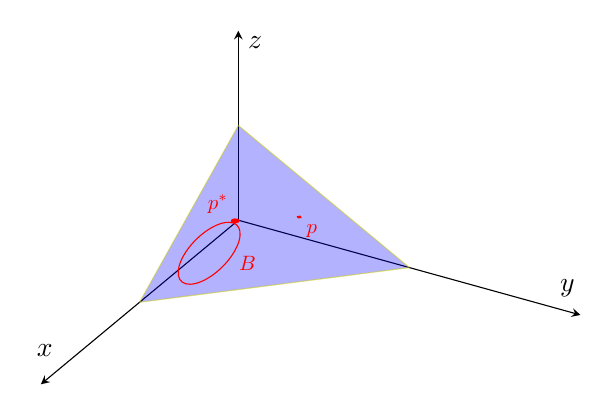
\begin{tikzpicture}
        \begin{axis}[
                axis lines = middle,
                xlabel = $x$,
                ylabel = $y$,
                zlabel = $z$,
                xtick=\empty,
                ytick=\empty,
                ztick=\empty,
                xmin = 0, xmax = 2,
                ymin = 0, ymax = 2,
                zmin = 0, zmax = 2,
                view={120}{45}
            ]
            \addplot3[
                patch,
                patch type=triangle,
                opacity=0.5,
                fill opacity=0.3,
                color=blue,
            ] coordinates {
                    (1, 0, 0)
                    (0, 1, 0)
                    (0, 0, 1)
                };

            % Draw a patch B on the surface 
            \node[red, scale=0.75] at (axis cs: 0.5, 0.25, 0.25) [below right] {$B$};
            \draw[red] (axis cs: 0.5, 0.25, 0.25) ellipse [x radius=0.2, y radius=0.2, rotate around={45:(axis cs: 0.5, 0.25, 0.25)}];

            % Plot random point p outside B 
            \draw[red, fill] (axis cs: 0.25, 0.5, 0.5) circle (0.01) node[below right, scale=0.75] {$p$};

            % Plot distinct point q 
            \draw[red, fill] (axis cs: 0.1, 0.04, 0.1) circle (0.02) node[above left, scale=0.75] {$p^*$};
        \end{axis}

    \end{tikzpicture}
\end{center}

\begin{tbox}{\textbf{Sanov's Theorem:} Let $B$ be an open subset of the space of all PMF on $\{1, \dots, s\}$. Then
        \[\lim_{n \to \infty} \frac{1}{n}\log \P(\hat p \in B) = -\inf_{q \in B} D(q \parallel p)\]
        Further, if $p^* = \argmin_{q \in B} D(q \parallel p)$ is unique, then
        \[\lim_{n \to \infty} \P(\norm{\hat p - p^*} > \ep \; | \; \hat p \in B) = 0 \quad \forall \ep > 0\]
        where $\norm{\hat p - p^*}$ is any metric, say $\norm{\hat p - p^*} = \max_{x \in \{1, \dots, s\}} \abs{\hat p_x - p_x}$}
    \emph{Proof:}
\end{tbox}

\tbf{Remark:} What if $p \in B$? Then $\inf_{q \in B} D(q \parallel p) = 0$, so
\[\frac{1}{n} \log \underbrace{e^{-o(n)}}\P(\hat p \in B) = 0\]


\section{Feb 5}
\tbf{Recall (Sanov's Theorem):} For $B$ open,
\begin{enumerate}
    \item \[\lim_{n \to \infty} \frac{1}{n} \log \P(\hat p_{x_1, \dots, x_n} \in B) = -\inf_{q\in B} D(q \parallel p)\]
    \item If $\exists ! \; p^* = \argmin_{q \in \bar B} D(q \parallel p)$, then
          \[\lim_{n \to \infty} \P(\norm{\hat p - p} > \ep \; | \; \hat p \in B) = 0 \quad \forall \ep >0 \]
\end{enumerate}


\begin{center}
    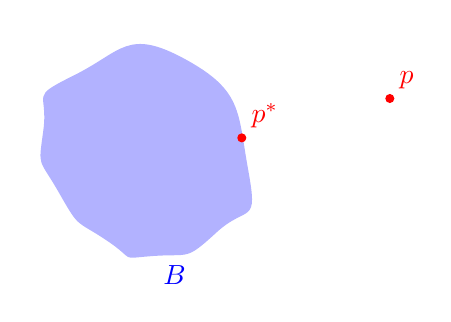
\begin{tikzpicture}
        % Draw a blob
        \fill[blue, opacity=0.3] plot[smooth cycle, tension=1.2] coordinates {
                (0, 0)
                (0.8, 0.3)
                (1.2, 1.1)
                (0.4, 2.5)
                (-1, 2.3)
                (-1.4, 1.6)
                (-1.2, 0.8)
                (-0.6, 0.2)
            };

        \draw[fill, red] (1.12, 1.5) circle (0.05) node[above right] {$p^*$};
        \draw[fill, red] (3, 2) circle (0.05) node[above right] {$p$};

        \node[blue, below right] at (0, 0) {$B$};
    \end{tikzpicture}
\end{center}

This leads to some interesting questions:
\begin{enumerate}
    \item Why is $p^*$ drawn on the boundary?
    \item Is there a case when $p^*$ lies in the interior?
\end{enumerate}

For the second: yes, if $p \in B$ (in which case $p$ is the global minimizer of $D(q \parallel p)$).

For the first, it suffices to show that since $D(q \parallel p)$ is a convex function, on any set $B$ with $p \notin B$, the minimizer $p^*$ must lie on the boundary.

\emph{Example:}

\begin{center}
    \begin{tikzpicture}
        \begin{axis}[
                axis lines = middle,
                xlabel = $x$,
                ylabel = $y$,
                xtick=\empty,
                ytick=\empty,
                clip=false
            ]
            \addplot[blue, domain=-4:1] {x^2 + 1};
            \addplot[red, dashed, domain=1:2] {x^2 + 1};
            \addplot[blue, domain=2:4] {x^2 + 1};


            \addplot[red, ultra thick, dashed, domain=1:2] {0} node[below] {$B$};

            \coordinate (A) at (0, 1);

            \coordinate (B) at (1, 2);

        \end{axis}
        \draw[blue, fill] (A) circle (0.1) node[above left] {$p$};
        \draw[red] (B) circle (0.1) node[above] {$p^*$};
    \end{tikzpicture}
\end{center}

\emph{Example:} $B = \{q \; | \; \exists x: \abs{q_x - p_x} > 0\}$

By Sanov,
\[\P(\hat p_n \in B) \approx \exp(-n \inf_{q\in B} D(q \parallel p)) \leq e^{-n/2} < 10\%\]

Now let's prove the claim:
\begin{proof}
    \emph{Proof:}
    \begin{align*}
        F(q)                                              & = D(q \parallel p) = \sum q_x \log \frac{p_x}{q_x} \\
                                                          & = \sum q_x \log q_x - \sum q_x \log p_x            \\
        \frac{\partial F}{\partial q_x}                   & = \log q_x + 1 - \log p_x                          \\
        \frac{\partial^2 F}{\partial q_x \, \partial q_y} & = \begin{cases}
                                                                  1/q_x & x = y    \\
                                                                  0     & x \neq y
                                                              \end{cases}                                 \\
        H                                                 & = \begin{pmatrix}
                                                                  \frac{1}{q_1}                             \\
                                                                   & \frac{1}{q_2}                          \\
                                                                   &               & \ddots                 \\
                                                                   &               &        & \frac{1}{q_s}
                                                              \end{pmatrix}
    \end{align*}
    But $\forall v \in \R^s$, $v^T H v = \sum v_i^2 \frac{1}{q_i} \geq 0 \implies H$ is positive semi-definite. Hence $F$ is convex.
\end{proof}

\subsection{Back to Gibbs' Heat Bath}
Recall the original motivating example where $X_1, \dots, X_n \sim p$, and $\frac{1}{n} \sum_{i=1}^{n} \Ec(X_i) = \theta$.

Previosuly, we showed that $\theta = \frac{1}{n} \sum_{i=1}^{n} \Ec(X_i) = \E_{\hat p} [\Ec(X)]$.

Now consider the set $B = \{q \; | \; \E_q [\Ec(X)] > \theta\}$ and define $\Omega = \{q: \E_q [\Ec(X)] = \theta\}$.

\begin{center}
    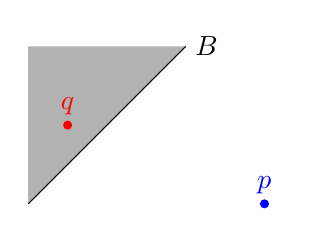
\begin{tikzpicture}
        \fill[opacity=0.3] plot coordinates {
                (0, 0)
                (2, 2)
                (0, 2)
            };

        \draw[fill, red] (0.5, 1) circle (0.05) node[above] {$q$};
        \draw (0, 0) -- (2, 2) node[right] {$B$};

        \draw[fill, blue] (3, 0) circle (0.05) node[above] {$p$};
    \end{tikzpicture}
\end{center}
Imagine we observe some sample with energy higher than expected (i.e. $q \in B$). What is the probability of this occuring?

By Sanov, in order to find $\inf_{q \in B} D(q \parallel p)$, it suffices to find $p^*$ such that $D(p^* \parallel p) = \inf_{q \in B} D(q \parallel p)$.

In the past, we used Lagrange multipliers to confirm our solution is in the \tbf{exponential family}
\[p_x^* = \frac{1}{Z_{\lambda}} p_x \exp(\lambda \Ec(x)) \quad \forall x\]
for some $\lambda$.

\emph{Example of Exponential Family:} $\mathcal{N}(\mu, \sigma^2)$ has PDF $\frac{1}{Z} e^{-\frac{(x- \mu)^2}{2\sigma^2}}$

If instead we had many constraints $\E_{\hat p} [\Ec_i(X)] = \theta_i$ for $i = 1, \dots, k$, we found minimizer
\[p^* = \frac{1}{Z_{\lambda_1 \dots \lambda_k}} p_x \exp(\lambda_1 \Ec_1(x) + \dots + \lambda_k \Ec_k(x))\]
where we found $\lambda_1, \dots, \lambda_k$ using Lagrange multipliers to satisfy the constraints and
\[Z_{\lambda_1\dots \lambda_k} = \sum_x p_x \exp(\lambda_1 \Ec_1(x) + \lambda_k \Ec_k(x))\]

These must also satisfy:
\begin{enumerate}
    \item $\frac{\partial}{\partial \lambda_k} \log Z_k = \E_{\lambda}[\Ec_k(X)]$
    \item $\frac{\partial^2}{\partial \lambda_k \lambda_l} \log Z_k = \text{Cov}_{\lambda}(\Ec_k(X), \Ec_l(X)) \quad \forall k, l$
    \item $\log Z_k$ is a convex function of $\lambda$ and it is strictly convex unless $\exists \alpha = (\alpha_1, \dots, \alpha_k)$ such that $\alpha \neq 0$ and $\sum_{k=1}^c \alpha_k \Ec_k(x) = \text{const} \quad \forall x$
    \item $\log Z_{\lambda} - \sum \lambda_k \theta_k$ is convex in $\lambda$ and minimized when $\E_{\lambda}[\Ec(X)] =\theta_k$
\end{enumerate}
\end{document}